\documentclass{standalone}
\usepackage{preset}
\begin{document}
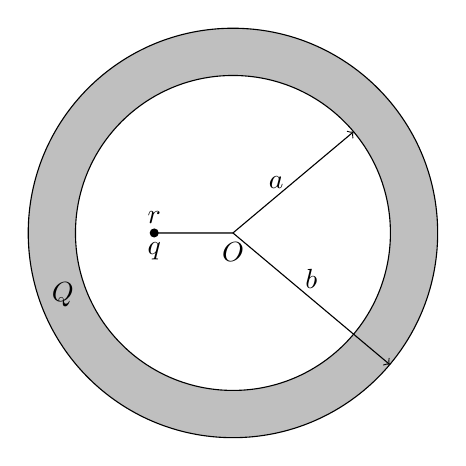
\begin{tikzpicture}[x=10mm,y=10mm]
	\draw[fill=lightgray](0,0)circle(2.6);
	\draw[fill=white](0,0)circle(2);
	\draw(0,0)node[below]{$O$};
	\draw[fill=black](0,0)--(-1,0)circle(.05)node[below]{$q$}node[above]{$r$};
	\draw[->](0,0)--node[above]{$b$}(-40:2.6);
	\draw[->](0,0)--node[left]{$a$}(40:2);
	\draw(200:2.3)node{$Q$};
\end{tikzpicture}
\end{document}
